%======================================================================
\chapter{Introduction}\label{ch:intro}
%======================================================================

\section{What this volume proves}

Volume~1 constructed a pseudo-arc in the plane: a nondegenerate continuum that is snake-like
(it can be covered by chains with arbitrarily small links) and hereditarily indecomposable
(every subcontinuum is indecomposable). This volume proves that there is essentially only one
pseudo-arc, and that it is homogeneous. These are the two facts about the pseudo-arc that the
classification of homogeneous plane continua needs.

Recall that the \emph{composant} of a point $p$ in a continuum $M$ is the union of all proper
subcontinua of $M$ that contain $p$ (Chapter~\ref{ch:composants}).

\begin{theorem}[Uniqueness of the pseudo-arc]\label{thm:intro-unique}
Any two pseudo-arcs are homeomorphic. More precisely, let $M$ and $M'$ be pseudo-arcs (in
possibly different metric spaces), let $p,q\in M$ lie in different composants of $M$, and let
$p',q'\in M'$ lie in different composants of $M'$. Then there is a homeomorphism $h\colon M\to
M'$ with $h(p)=p'$ and $h(q)=q'$.
\end{theorem}

\begin{theorem}[Homogeneity of the pseudo-arc]\label{thm:intro-homog}
For any two points $p,q$ of a pseudo-arc $M$ there is a homeomorphism $h\colon M\to M$ with
$h(p)=q$.
\end{theorem}

\begin{corollary}\label{cor:intro}
\begin{enumerate}[label=(\alph*)]
\item Every pseudo-arc is homeomorphic to the pseudo-arc in the plane constructed in
Volume~1.
\item Every nondegenerate subcontinuum of a pseudo-arc is a pseudo-arc, and hence is
homeomorphic to the whole pseudo-arc.
\end{enumerate}
\end{corollary}

These results are due to R.~H.~Bing (1948 and 1951). Theorem~\ref{thm:intro-unique} for
the continua described by sequences of crooked chains is Theorem~12 of his 1948 paper; the
fact that every pseudo-arc has such a description, so that the theorem applies to all
pseudo-arcs, is Theorem~1 of his 1951 paper ``Concerning hereditarily indecomposable
continua''. As in Volume~1, the notes follow the formal proof rather than the papers; the main
differences are listed in Section~\ref{sec:intro-diff}.

\section{The shape of the proof}

The proof has three parts.

\paragraph{Part I: two descriptions give a homeomorphism (Chapters~\ref{ch:patterns}--\ref{ch:two}).}
A \emph{description} from $P$ to $Q$ is a sequence of chains $D^{(0)},D^{(1)},\dots$ from $P$ to
$Q$, each crooked in the one before, with closures of links nested and mesh tending to zero
(\vone{Definition~3.1}). Its \emph{described set} is $M=\bigcap_i\bigcup D^{(i)}$. We prove:

\begin{quote}
\emph{If two descriptions, from $P_1$ to $Q_1\ne P_1$ and from $P_2$ to $Q_2\neq P_2$, live in
compact metric spaces, then there is a homeomorphism between the described sets taking $P_1$
to $P_2$ and $Q_1$ to $Q_2$.}
\end{quote}

The idea is to build, alternately in the two spaces, two sequences of chains with the same
numbers of links which ``follow the same patterns'' in each other. Two ingredients are
needed.
\begin{itemize}
\item \emph{Pattern following} (Chapter~\ref{ch:patterns}): given any pattern, that is, any walk
$x$ through the links of a level $D^{(i)}$ from its first link to its last, some deeper level
can be grouped into a chain that follows $x$. The proof is a purely combinatorial statement
about integer sequences, proved by induction, and a compactness argument.
\item \emph{Matching covers} (Chapter~\ref{ch:matching}): if two compact sets carry sequences of
finite open covers, indexed in the same way, such that ``the $j$-th set of one level meets the
$k$-th set of the level before'' on one side forces the corresponding sets on the other side to
be close, then the two compact sets are homeomorphic. This is a general metric statement with
no chains in it.
\end{itemize}
Chapter~\ref{ch:two} combines them.

\paragraph{Part II: every pseudo-arc has a description (Chapters~\ref{ch:folding}--\ref{ch:descriptions}).}
Let $M$ be a pseudo-arc and let $p,q\in M$ lie in different composants. We prove:

\begin{quote}
\emph{In the compact space $M$ there is a description from $p$ to $q$ whose described set is
all of $M$.}
\end{quote}

The proof has two halves. First (Chapter~\ref{ch:descriptions}, following Bing's 1951
argument) hereditary indecomposability forces fine chains covering $M$ to be crooked in coarse
ones; this gives a sequence of chains, each crooked in the previous one, but not yet going from
$p$ to $q$. Second, each chain must be replaced by one that goes from $p$ to $q$. For this one
needs a theorem about crooked chains alone:

\begin{itemize}
\item \emph{The folding theorem} (Chapter~\ref{ch:folding}, Bing's Theorem~4): if a chain $E$ is
crooked in a chain $D$, and a stretch of $E$ from a link $r$ to a link $s$ reaches both end links
of $D$, then the links of $E$ can be grouped into consecutive blocks forming a chain, with $r$ in
the first block and $s$ in the last, and every block inside three consecutive links of $D$.
\end{itemize}

This is the longest proof of the volume. It is again purely combinatorial: it is a statement
about an integer sequence (the indices of the links of $D$ containing the successive links of
$E$) that moves by at most one at each step and is ``crooked''.

\paragraph{Part III: composants and the main theorems (Chapters~\ref{ch:composants} and
\ref{ch:main}).}
To apply Parts~I and~II one needs two points in different composants. Chapter~\ref{ch:composants}
proves that in an indecomposable continuum no composant is the whole continuum; so every point
$p$ of a pseudo-arc has a point $q$ outside its composant. Chapter~\ref{ch:main} assembles the
proofs of Theorems~\ref{thm:intro-unique} and~\ref{thm:intro-homog} and of
Corollary~\ref{cor:intro}.

\medskip
The logical dependence of the chapters is:
\begin{center}
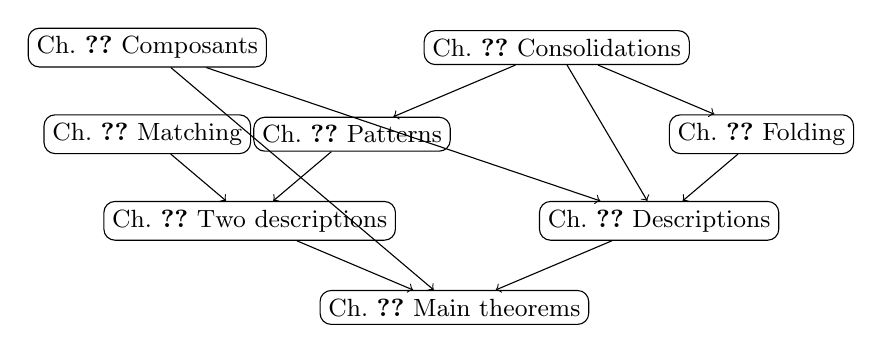
\begin{tikzpicture}[x=2.6cm,y=1.1cm,every node/.style={draw,rounded corners,inner sep=3pt,font=\small}]
\node (c1) at (0,2) {Ch.~\ref{ch:composants} Composants};
\node (c2) at (2,2) {Ch.~\ref{ch:consolidations} Consolidations};
\node (c3) at (1,1) {Ch.~\ref{ch:patterns} Patterns};
\node (c4) at (0,1) {Ch.~\ref{ch:matching} Matching};
\node (c5) at (0.5,0) {Ch.~\ref{ch:two} Two descriptions};
\node (c6) at (3,1) {Ch.~\ref{ch:folding} Folding};
\node (c7) at (2.5,0) {Ch.~\ref{ch:descriptions} Descriptions};
\node (c8) at (1.5,-1) {Ch.~\ref{ch:main} Main theorems};
\draw[->] (c2) -- (c3); \draw[->] (c2) -- (c6); \draw[->] (c3) -- (c5); \draw[->] (c4) -- (c5);
\draw[->] (c6) -- (c7); \draw[->] (c2) -- (c7); \draw[->] (c1) -- (c7);
\draw[->] (c5) -- (c8); \draw[->] (c7) -- (c8); \draw[->] (c1) -- (c8);
\end{tikzpicture}
\end{center}

\section{Where the formal proof differs from the papers}\label{sec:intro-diff}

The formal proof follows Bing's architecture. It departs from his text in the following
places, and the notes follow the formal proof.

\begin{enumerate}
\item \textbf{Pattern following needs $P\neq Q$.} Bing's Theorem~6 (pattern following) is false
for a description of a one-point space, where $P=Q$ (Remark~\ref{rem:pf-false}); the formal
proof adds the hypothesis $P\ne Q$, which is harmless since the uniqueness theorem assumes it
anyway.
\item \textbf{Pattern following is proved directly}, from a combinatorial statement about
integer sequences (Theorem~\ref{thm:realize}) whose induction is designed to be checkable. Bing
derives Theorem~6 from a more general Theorem~5, whose proof leaves a step to the reader.
\item \textbf{Compactness of the ambient space.} Bing's uniqueness theorem asks only that the
described sets be compact. That is not enough: there is a description, in a non-complete
space, whose described set is compact but not connected (\vone{Remark~3.5}). The formal
statement asks that the links lie in a compact set (equivalently, after restricting, that the
ambient space be compact).
\item \textbf{The folding theorem with three links.} Bing's Theorem~4 asks that every block lie
in the union of \emph{two} adjacent links of $D$, and derives it from his Theorem~3. The formal
proof proves the version with \emph{three} consecutive links directly, by a ``greedy zigzag''
construction (Chapter~\ref{ch:folding}), which is all that the later arguments use: they only
need the blocks to be small. It also proves the version, needed for chains from a point $R$ to
a point $S$, in which $R$ may lie in two adjacent links.
\item \textbf{Crookedness of fine chains} (Bing 1951, first paragraph of the proof of
Theorem~1) is proved by a limit argument whose witnesses are chosen so that the two limit
continua are visibly not nested (Section~\ref{sec:crooked-eventually}).
\end{enumerate}

\section{Prerequisites and conventions}

The reader should know Volume~1, in particular Chapters~1--3: chains, refinements, crookedness,
descriptions, and the theorem that a described set is a pseudo-arc. References to Volume~1 are
written ``\vone{Lemma~2.5}''. The numbering of Volume~1 starts with Chapter~0 (the
introduction), as here. We use the conventions of Volume~1:

\begin{itemize}
\item $\N=\set{0,1,2,\dots}$, and $[n]=\set{0,1,\dots,n-1}$. Chains are indexed from $0$.
\item A \emph{chain} of length $n$ is a sequence $D=(D_0,\dots,D_{n-1})$ of open sets (links)
with $D_i\cap D_j\neq\emptyset$ if and only if $\abs{i-j}\le1$ (\vone{Definition~2.1}). A chain
\emph{goes from $P$ to $Q$} if $P$ lies in the first link and in no other, and $Q$ lies in the
last link and in no other.
\item ``Crooked'' always means crooked in the sense of \vone{Definition~2.11}: $E$ is crooked
in $D$ if $E$ refines $D$ and, whenever $k>h+2$ and $E_i$ meets $D_h$ and $E_j$ meets $D_k$, there
are $r,s$ strictly between $i$ and $j$, with $r$ nearer to $i$, such that $E_r\subseteq D_{k-1}$
and $E_s\subseteq D_{h+1}$.
\item A function $g$ defined on a set of consecutive integers has \emph{unit steps} if
$\abs{g(t+1)-g(t)}\le1$ whenever both sides are defined.
\end{itemize}

\paragraph{Formal counterparts.} As in Volume~1, many results are followed by a line
``Formal counterpart:'' naming the corresponding declaration of the Lean development (all names
begin with \lean{HPC.}). These lines may be skipped. Appendix~\ref{app:formal} collects them.

\paragraph{Exercises.} Each chapter ends with exercises. None of them is used later.
